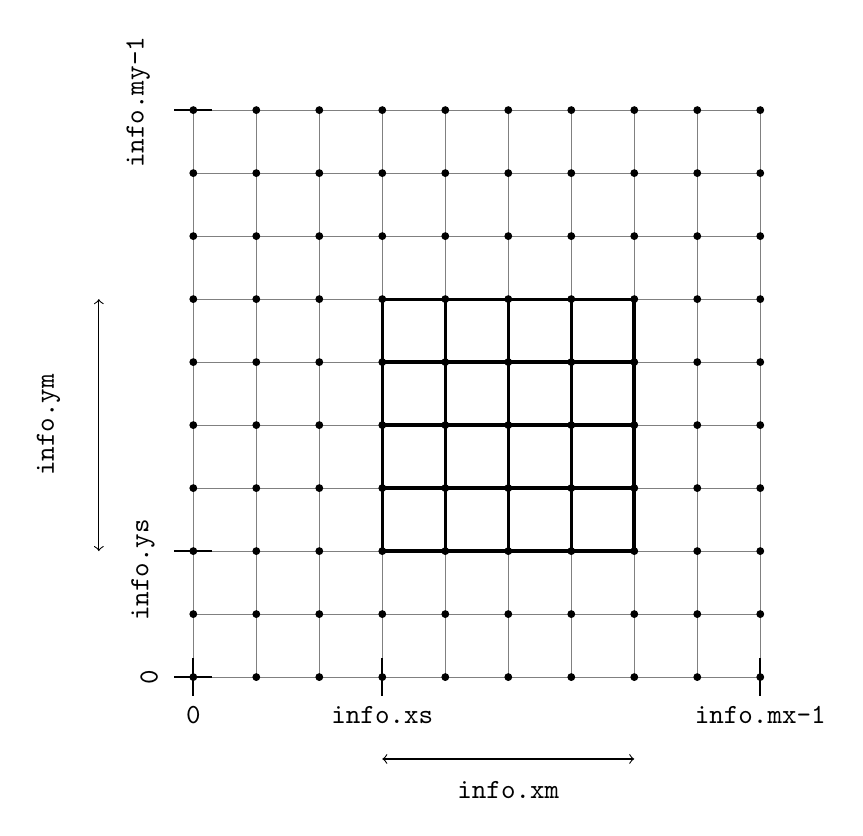
\begin{tikzpicture}[scale=8]
  % global grid, local grid, nodes
  \draw[xstep=0.1,ystep=0.1,gray,very thin] (0.0,0.0) grid (0.9,0.9);
  \draw[xstep=0.1,ystep=0.1,black,very thick] (0.3,0.2) grid (0.7,0.6);
  \foreach \y in {0,...,9}
    \foreach \x in {0,...,9} {
      \filldraw (\x * 0.1,\y * 0.1) circle (0.15pt);
    }
  % ticks on x-axis at 0, xs, mx
  \draw[black,thick] (0,-0.03)   -- (0,+0.03);
  \draw[black,thick] (0.3,-0.03) -- (0.3,+0.03);
  \draw[black,thick] (0.9,-0.03) -- (0.9,+0.03);
  \node at (0,-0.06) {\texttt{0}};
  \node at (0.3,-0.06) {\texttt{info.xs}};
  \node at (0.9,-0.06) {\texttt{info.mx-1}};
  % ticks on y-axis at 0, ys, my
  \draw[black,thick] (-0.03,0)   -- (+0.03,0);
  \draw[black,thick] (-0.03,0.2) -- (+0.03,0.2);
  \draw[black,thick] (-0.03,0.9) -- (+0.03,0.9);
  \node[rotate around={90:(0,0)}] at (-0.07,0) {\texttt{0}};
  \node[rotate around={90:(-0.2,0.2)}] at (-0.08,0.12) {\texttt{info.ys}};
  \node[rotate around={90:(0.0,0.9)}] at (-0.20,0.8) {\texttt{info.my-1}};
  % xm, ym along sides of local patch
  \draw[<->,] (0.3,-0.13) -- (0.7,-0.13);
  \node at (0.5,-0.18) {\texttt{info.xm}};
  \draw[<->,] (-0.15,0.2) -- (-0.15,0.6);
  \node[rotate around={90:(0.3-0.3,0.4)}] at (-0.28,0.35) {\texttt{info.ym}};
\end{tikzpicture}

